\documentclass[a4paper]{article}
\usepackage{fullpage}
\usepackage{hyperref}
\usepackage{url}
\usepackage{amssymb}
\usepackage{graphicx}
\usepackage[margin=1in]{geometry}
%\usepackage{polski}
\usepackage[utf8]{inputenc}


\setlength{\parindent}{0pt}
\addtolength{\parskip}{\baselineskip}

\title{TANR (Twitter Augmented News Reader)\\Executive Summary\\}

\author{
    \small{Rafał Szymański}\\
  	\and
    \small{Maciek Albin}\\
    \and
    \small{Sam Wong}\\
    \and  
    \small{Suhaib Sarmad}\\
		\and
		\small{Jamal Khan}\\
		\and
		\small{\{rs2909, mja108, sw2309, sss308, jzk09\}@doc.ic.ac.uk}
		\and
}

\date{}

\begin{document} 
	\maketitle
	
  \section{High Level Overview}
  
  Twitter Augmented News Reader - A webapp that pairs current news with relevant tweets.
  
  Traditionally, the media has been presenting news stories biased with the writers’ point of view or agenda, recruiting readers to join their agendas. This webapp presents a balanced view to the readers. We pair up relevant tweets to news emerging around the world, analyse the sentiment value of those tweets, and display this information in a minimalistic and visually appealing user interface. Our aim is to create a new kind of news reader that not only presents a new story, but also the social discussion behind it.
  
  \section{Technical Overview}
  
  \begin{center}
	 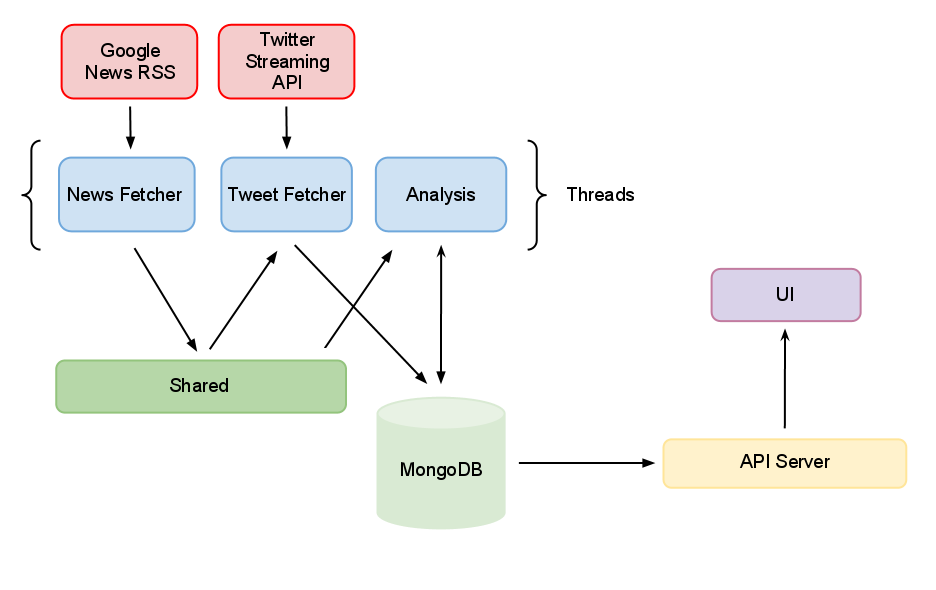
\includegraphics[scale=0.35]{infrastructure.png}
  \end{center}
	 
	 	We decided to divide the project into two separate technical parts: \emph{Analysis} and \emph{UI}, that would be connected through our own \emph{API} server
	 	
	 	\emph{Analysis} process is divided into three separate threads:
  	\begin{description}
  	 \item[News Fetcher] responsible for fetching current news stories from an RSS feed, getting information relevant to us, and generating keywords
  	 \item[Tweet Fetcher] responsible for fetching tweets using keywords generated by \emph{News Fetcher}
  	 \item[Analysis] uses tweets gathered by \emph{Tweet Fetcher} and info gathered by \emph{News Fetcher} to calculate Twitter's reaction to news stories
  	\end{description}
	 
	 The API provides a very thin layer between the \emph{UI} and the data stored in the database. It's written in Python using Flask and the API calls return results in JSON.
	 
	 The UI connects to the server's API and displays the information in a tiled layout. These tiles dynamically rearrange themselves and adjust to the size of the users' window or screen. Each tile displays an image related to the article and title of the article. On hover/click of a tile, the image folds away, revealing the details: a short summary, a word cloud made from common words found in relevant tweets, a list of relevant tweets and the overall sentiment.
  
  \section{Software Engineering Issues}
  
	The initial idea of the project was related to analysing a follower graph of a subset of Twitter users influential in a certain topic of interest. Limitations in the Twitter API, such as limited number of calls per hour, prevented the continuation of this idea, and caused an idea pivot. The new project became augmenting news with reactions expressed by users of Twitter.
  
	While the project certainly had its technical issues and challenges, group and team management problems also emerged. We learned about working in teams and how teams can make or break whether a project is successful or not. 
	
	We quickly experienced the effect of not assigning to clear roles to each group member, and having an authority to supervise and ensure the execution of these task assignments. Initially, all group members were trying to cover too many points. This was solved by using Trello\footnote{\url{http://trello.com}, software that allows to assign tasks to team members}, which helped settle the responsibilities of each group member, and ensure their timely execution.
	
  
  \section{Validation and Conclusions}
  
	From time to time we asked for feedback on the user facing products. This was done so that we could make design and functionality choices. For example, we talked to our supervisor Jeremy Bradley, and he liked our user interface but wanted us to add pictures for each news story. We took his advice and implemented it. This has resulted very positive feedback in subsequent feedbacks.
	
	We used Pylint4 to validate the Python code which we wrote. This was done to check for errors such as incorrect indentation, bad naming conventions for class names and functions, among others. Checking for errors and validating the UI side of the project was done using the W3 Validator.
	
	We conclude that this project was a good exercise in learning software development techniques, and exposing problems related to working in a group. The resulting end product is successful, and presents news stories along with their related tweets and sentiment analysis, in a visually appealing and minimalistic UI.
  

\end{document}
